\documentclass[border=12pt]{standalone}
\usepackage[utf8]{inputenc}
\usepackage[dvipsnames]{xcolor}
\usepackage{amsmath}
\usepackage{amssymb}
\usepackage{tikz}
\usetikzlibrary{arrows.meta,positioning}

\definecolor{schemagreen}{RGB}{198,239,206}  % final (green)
\definecolor{datafill}{RGB}{244,248,253}      % data state (pale blue)
\definecolor{normfill}{RGB}{255,236,204}      % normalization step (amber)
\definecolor{dbfill}{RGB}{231,222,242}        % DBpedia-only step (lavender)
\definecolor{dbedge}{RGB}{118,70,168}         % DBpedia-only border (purple)

\begin{document}
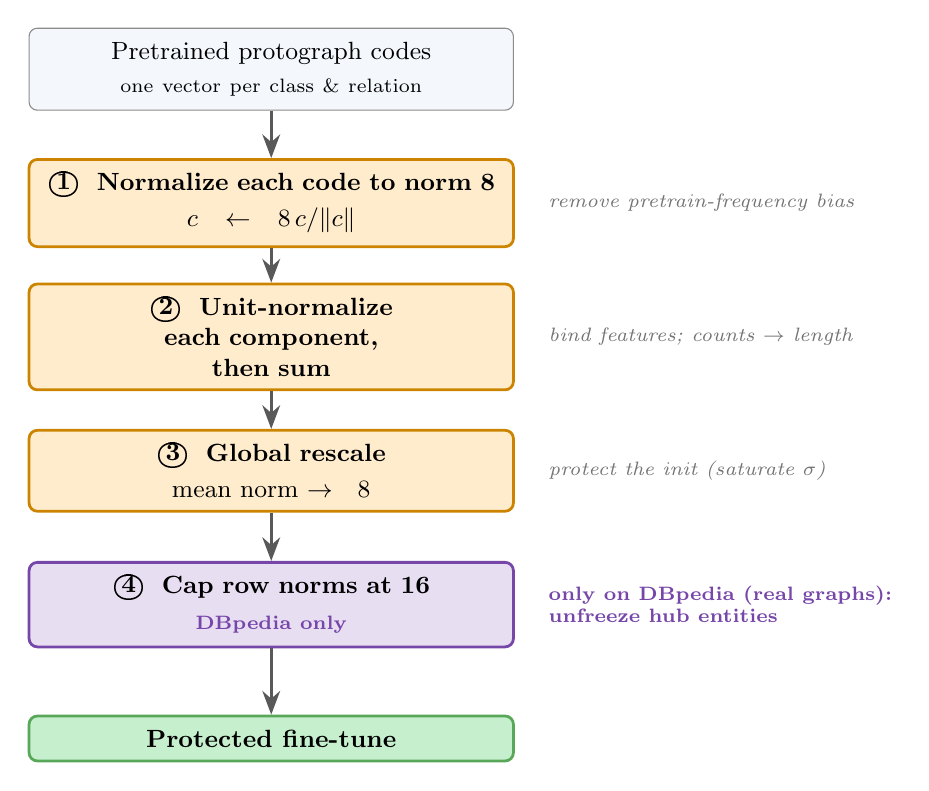
\begin{tikzpicture}[
  font=\small,
  data/.style ={rounded corners=3pt, draw=black!45, fill=datafill,
                text width=58mm, align=center, inner sep=5pt},
  op/.style   ={rounded corners=3pt, draw=Orange!80!black, line width=1pt,
                fill=normfill, text width=58mm, align=center, inner sep=5pt},
  dbop/.style ={rounded corners=3pt, draw=dbedge, line width=1pt,
                fill=dbfill, text width=58mm, align=center, inner sep=5pt},
  final/.style={rounded corners=3pt, draw=ForestGreen!75, line width=1pt,
                fill=schemagreen, text width=58mm, align=center, inner sep=5pt,
                font=\small\bfseries},
  note/.style ={anchor=west, font=\scriptsize\itshape, text=black!55},
  dbnote/.style={anchor=west, font=\scriptsize\bfseries, text=dbedge},
  flow/.style ={-{Stealth[length=3mm]}, line width=1.1pt, draw=black!65},
]

\node[data]  (codes) at (0,9.0) {Pretrained protograph codes\\[1pt]
  {\scriptsize one vector per class \& relation}};
\node[op]    (s1) at (0,7.3) {\textbf{\textcircled{1}\; Normalize each code to norm 8}\\[2pt]
  $c \leftarrow 8\,c/\lVert c\rVert$};
\node[op]    (s2) at (0,5.6) {\textbf{\textcircled{2}\; Unit-normalize each component,}\\
  \textbf{then sum}};
\node[op]    (s3) at (0,3.9) {\textbf{\textcircled{3}\; Global rescale}\\[2pt]
  mean norm $\to 8$};
\node[dbop]  (s4) at (0,2.2) {\textbf{\textcircled{4}\; Cap row norms at 16}\\[2pt]
  {\scriptsize\bfseries\textcolor{dbedge}{DBpedia only}}};
\node[final] (ft) at (0,0.5) {Protected fine-tune};

\draw[flow] (codes) -- (s1);
\draw[flow] (s1) -- (s2);
\draw[flow] (s2) -- (s3);
\draw[flow] (s3) -- (s4);
\draw[flow] (s4) -- (ft);

\node[note] at (3.4,7.3) {remove pretrain-frequency bias};
\node[note] at (3.4,5.6) {bind features; counts $\to$ length};
\node[note] at (3.4,3.9) {protect the init (saturate $\sigma$)};
\node[dbnote, align=left] at (3.4,2.2) {only on DBpedia (real graphs):\\ unfreeze hub entities};

\end{tikzpicture}
\end{document}
